\section{Aufbau und Durchführung}

\begin{figure}
    \begin{subfigure}{0.5\textwidth}
        \centering
        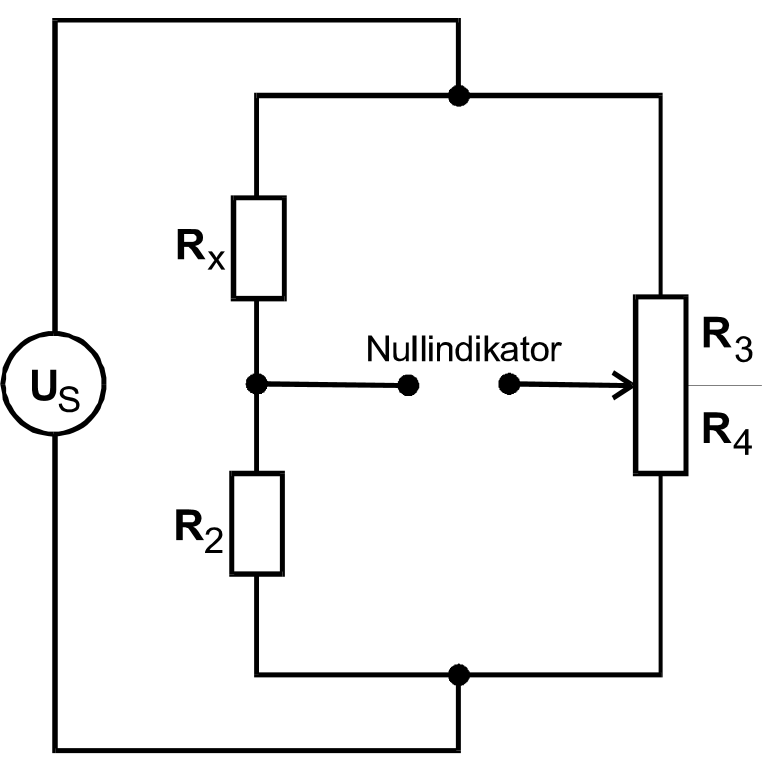
\includegraphics[height=5cm]{Bilder/Wheatstone.png}
        \caption{Wheatstonesche Brückenschaltung}
        \label{fig:Wheatstone}
    \end{subfigure}
    \begin{subfigure}{0.5\textwidth}
        \centering
        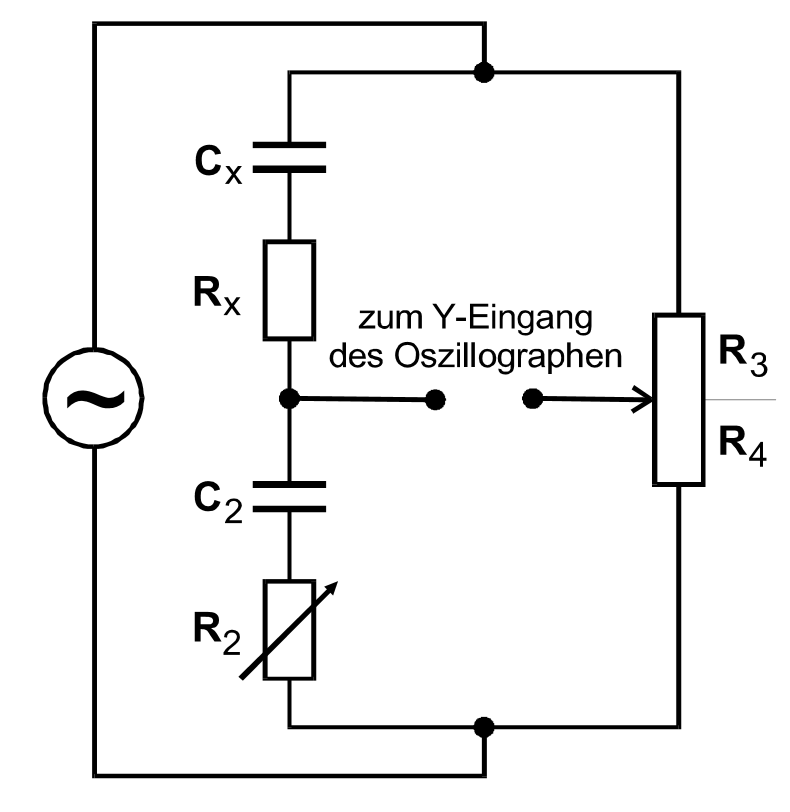
\includegraphics[height=5cm]{Bilder/Kapazitiv.png}
        \caption{Kapazitive Brückenschaltung}
        \label{fig:Kapazitiv}
    \end{subfigure}
    \begin{subfigure}{0.5\textwidth}
        \centering
        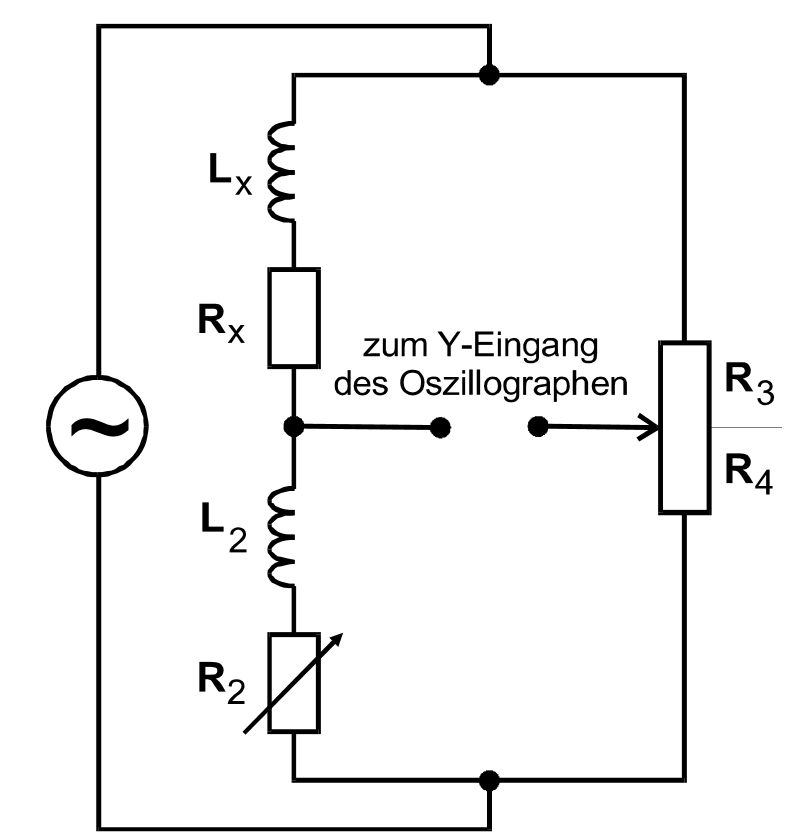
\includegraphics[height=5cm]{Bilder/Induktiv}
        \caption{Induktive Brückenschaltung}
        \label{fig:Induktiv}
    \end{subfigure}
    \begin{subfigure}{0.5\textwidth}
        \centering
        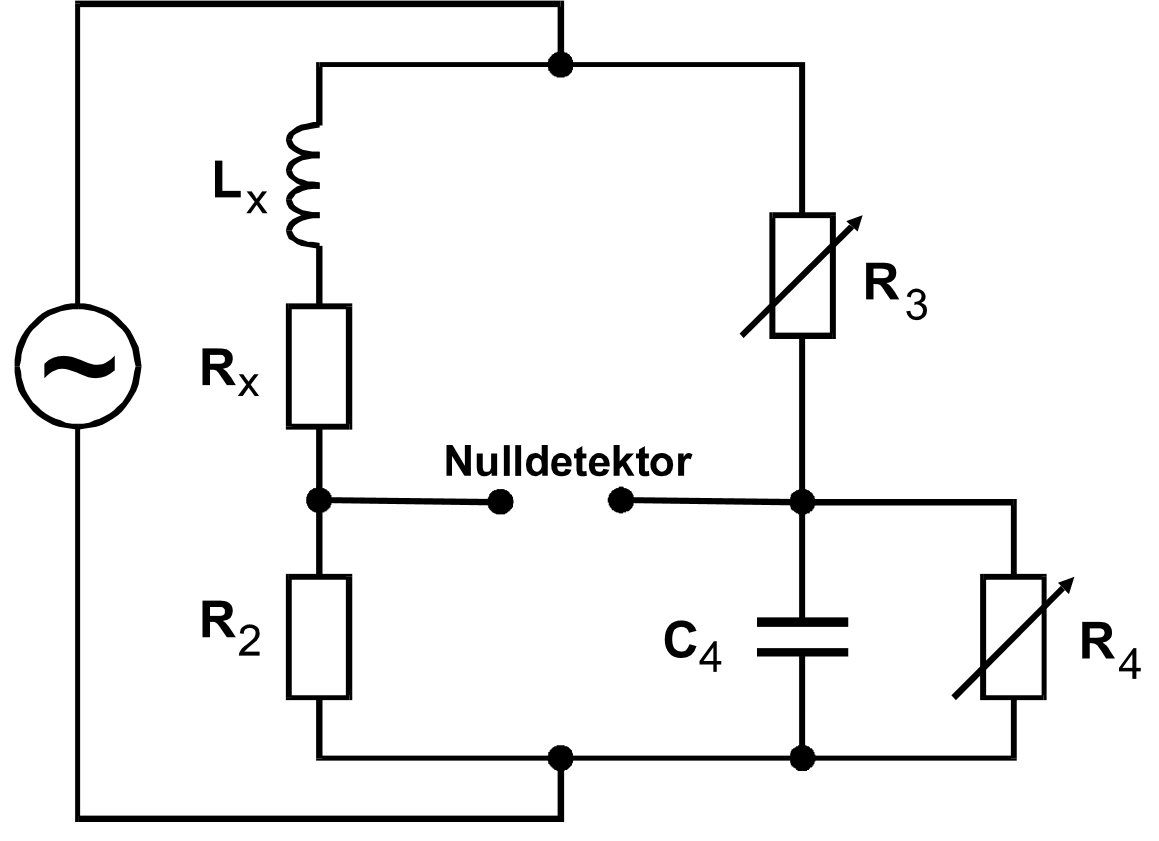
\includegraphics[height=5cm]{Bilder/Maxwell}
        \caption{Maxwellsche Brückenschaltung}
        \label{fig:Maxwell}
    \end{subfigure}
    \begin{subfigure}{0.5\textwidth}
        \centering
        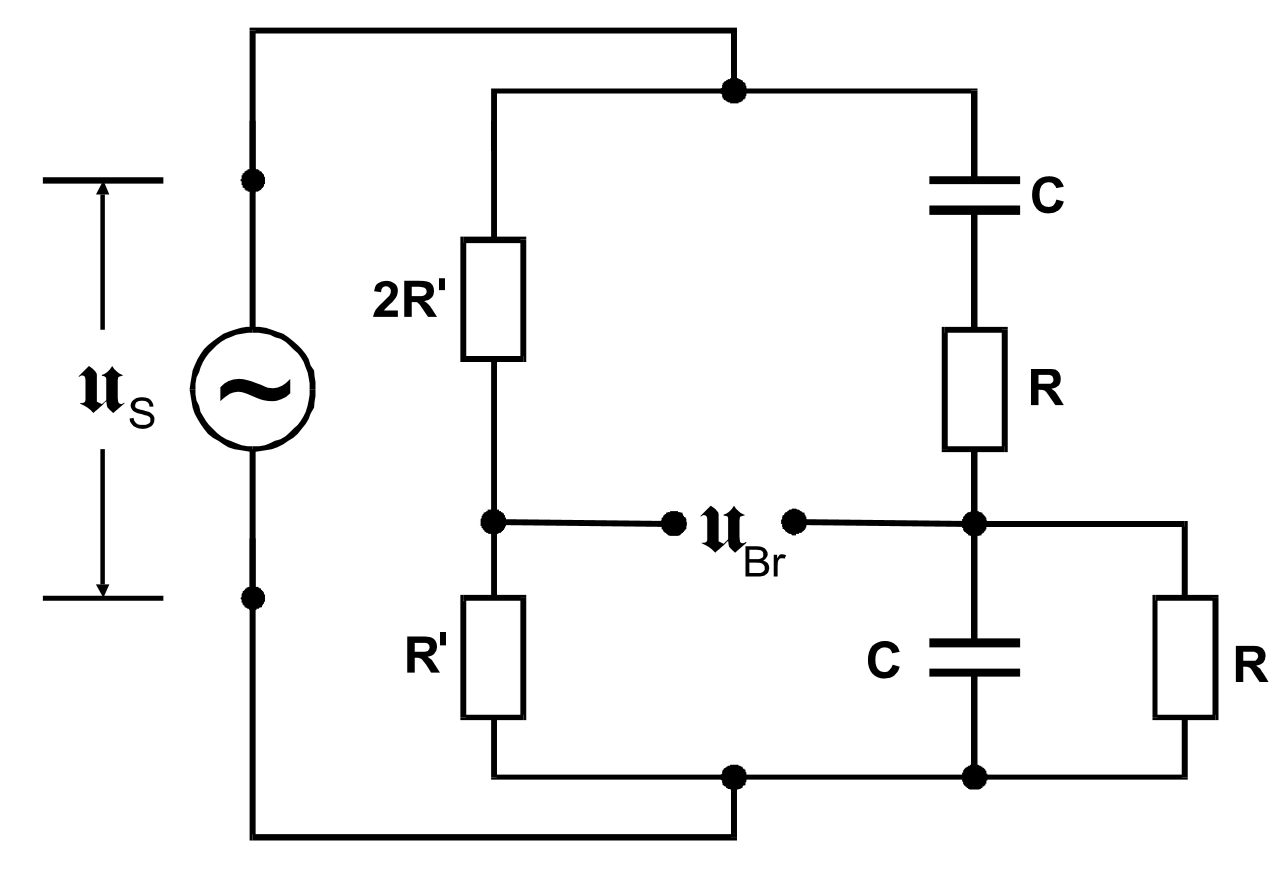
\includegraphics[height=5cm]{Bilder/Wien-Robinson}
        \caption{Wien-Robinson Brückenschaltung}
        \label{fig:Wien}
    \end{subfigure}
\end{figure}

\label{sec:Durchführung}
